\let\negmedspace\undefined
\let\negthickspace\undefined
\documentclass[journal]{IEEEtran}
\usepackage[a5paper, margin=10mm, onecolumn]{geometry}
%\usepackage{lmodern} % Ensure lmodern is loaded for pdflatex

\setlength{\headheight}{1cm} % Set the height of the header box
\setlength{\headsep}{0mm}     % Set the distance between the header box and the top of the text

\usepackage{gvv-book}
\usepackage{gvv}
\usepackage{cite}
\usepackage{amsmath,amssymb,amsfonts,amsthm}
\usepackage{algorithmic}
\usepackage{graphicx}
\usepackage{textcomp}
\usepackage{xcolor}
\usepackage{txfonts}
\usepackage{listings}
\usepackage{enumitem}
\usepackage{mathtools}
\usepackage{gensymb}
\usepackage{comment}
\usepackage[breaklinks=true]{hyperref}
\usepackage{tkz-euclide} 
\usepackage{listings}
% \usepackage{gvv}                                        
\def\inputGnumericTable{}                                 
\usepackage[latin1]{inputenc}                                
\usepackage{color}                                            
\usepackage{array}                                            
\usepackage{longtable}                                       
\usepackage{calc}                                             
\usepackage{multirow}                                         
\usepackage{hhline}                                           
\usepackage{ifthen}                                           
\usepackage{lscape}


\renewcommand{\thefigure}{\theenumi}
\renewcommand{\thetable}{\theenumi}
\setlength{\intextsep}{10pt} % Space between text and floats


\numberwithin{equation}{enumi}
\numberwithin{figure}{enumi}
\renewcommand{\thetable}{\theenumi}


% Marks the beginning of the document
\begin{document}
\bibliographystyle{IEEEtran}
\vspace{3cm}

\title{9.4.18}
\author{EE24BTECH11047 - Niketh Prakash Achanta}
% \maketitle
% \newpage
% \bigskip
{\let\newpage\relax\maketitle}
\renewcommand{\thefigure}{\theenumi}
\renewcommand{\thetable}{\theenumi}
\textbf{Question:} At any point $\brak{x,y}$ of a curve, the slope of the tangent is twice the slope of the line segment joining the point of contact to the point $\brak{-4,-3}$. Find the equation of the curve given that it passes through $\brak{-2,1}$.\\

\textbf{Solution}\\
    $\text{Slope of tangent} = \frac{dy}{dx}\\ 
    \text{Based on the given information, we can form the following differential equation:}$ \\
    \begin{align*}
    \frac{dy}{dx}=2\brak{\frac{y+3}{x+4}}     
    \end{align*}
Then, cross-mutliply 
    \begin{align*}
        \frac{dy}{y+3}=2\frac{dx}{x+4}
    \end{align*}
Integrate
    \begin{align*}
        \int{\frac{dy}{y+3}}=2\int{\frac{dx}{x+4}}
    \end{align*}
After integration
    \begin{align*}
        \ln{\brak{y+3}}=2\ln{\brak{x+4}}+k    
    \end{align*}
Where k is an arbitrary constant of integration.\\
Now, rewrite $2\ln{\brak{x+4}}$ as ${\ln{\brak{x+4}}}^2$ and take that term to LHS
    \begin{align*}
        \ln{\frac{\brak{y+3}}{{\brak{x+4}}^2}}=k\\
        \frac{\brak{y+3}}{{\brak{x+4}}^2}={e}^k
    \end{align*}
Replace $e^k$ with another constant "c"
    \begin{align*}
        y=c{\brak{x+4}}^2 - 3
    \end{align*}
Given that the curve passes through $\brak{-2,1}$ substitute $x=-2,y=1$ in the current equation
Thus, $c=1$\\
$\therefore$ Final Equation of the Curve: $y={\brak{x+4}}^2 - 3$

Additionally, a numerical solution is generated using the method of finite differences:
The derivative is approximated using finite differences:
	\begin{align*}
    \frac{dy}{dx}&=\frac{y(x+h)-y(x)}{h}\\
    y(x+h)&=y(x)+h\brak{\frac{dy}{dx}}
	\end{align*}
h is a value close to zero, that can be chosen accordingly while creating the program.\\
So we iterate as follows:
	\begin{align*}
		y_{n+1}=y_{n} + h\brak{\frac{dy}{dx}}
	\end{align*}
	\begin{align*}
		x_{n+1}=x_{n}+h
	\end{align*}
	\begin{align*}
		\text{Here, } \frac{dy}{dx}&=2\frac{\brak{y+3}}{\brak{x+4}}
	\end{align*}
We start with given point $\brak{-2,1}$. $x_{0}=-2$ and $y_{0}=1$. We iterate for a suitable number of times in order to get a solution that is approximately equal to the theoretical solution.
\begin{figure}[!ht]
    \centering
    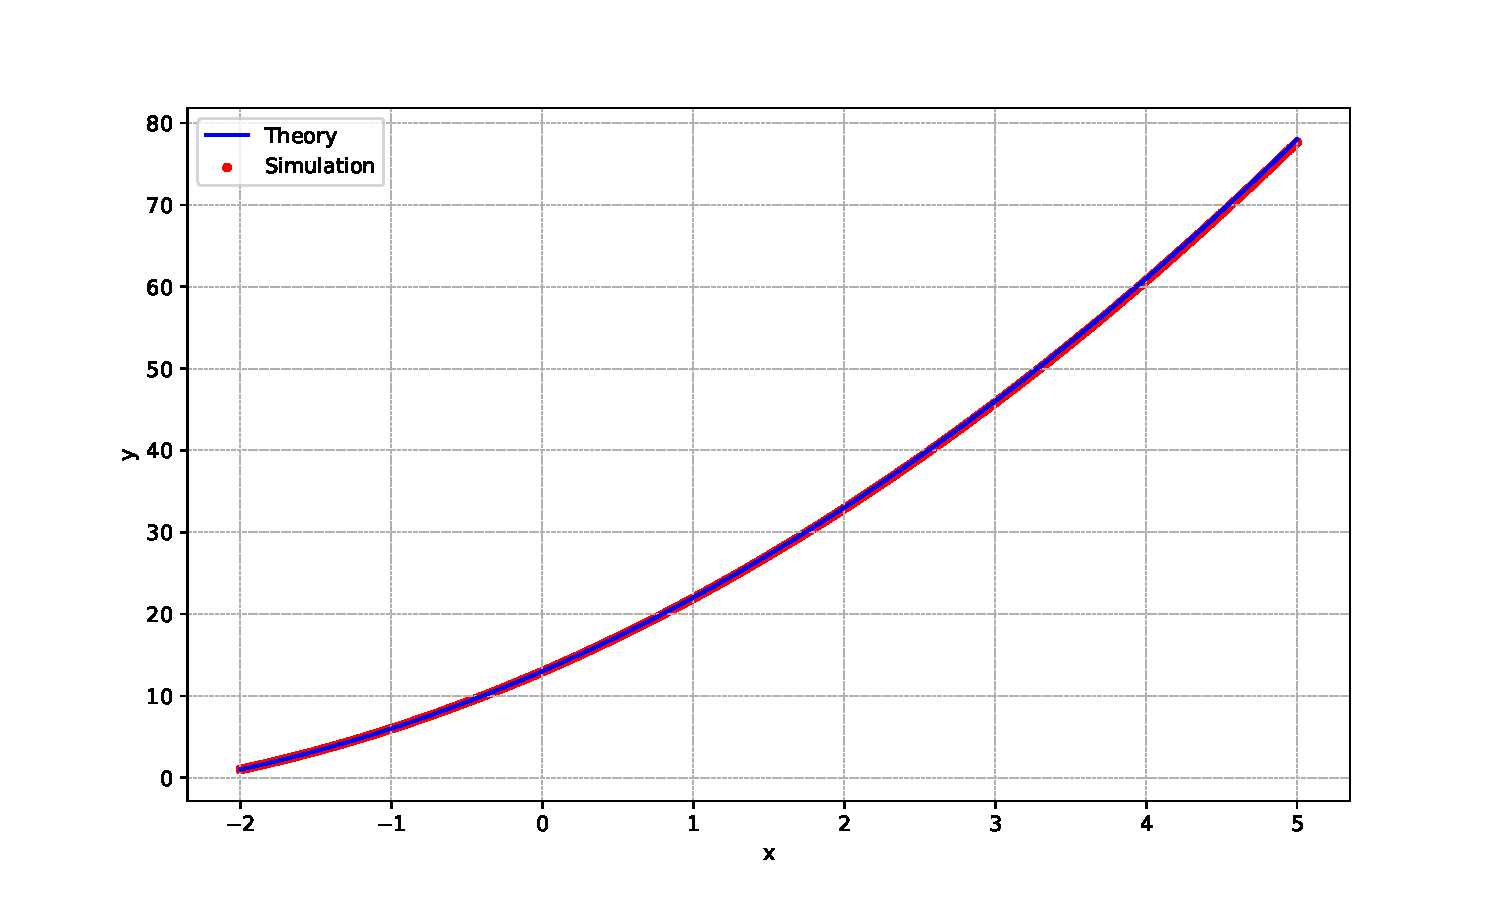
\includegraphics[width=\columnwidth]{/home/niketh/EE1003/Assignment-1/figs/comparison_plot.pdf}
    \caption{}
\end{figure}

\end{document}
